\section{The Sharp Gap and Its Extensions}\label{app:C}
\subsection{The Sharp Universal Gap}\label{app:universal}
We prove Theorem~\ref{thm:universal} and the program comparison
\begin{equation}
 \Phi_n(d,\A_{\rm fixed}(b))
 \le \Phi_{n/K_{m,b}}(d,\A_{\rm branch}(b)).
 \label{eq:programsimulation}
\end{equation}
Here the program is defined for any positive real sample-size argument.
All scores in the construction below depend only on the queried feature values; the estimator subsequently multiplies them by $Y$. Theorems~\ref{thm:finite} and~\ref{thm:asym} already compare these constructions with the larger class of history-dependent protocols, including branching choices based on the current label.

\subsubsection{Simulating One Tree without Branching}
Let $\tau$ be a deterministic tree of depth at most $b$ on $m\ge b$ coordinates, and let $H_\tau(x)$ be a score constant on each of its leaves. A repeated query on a path can be removed because its answer is already known. At every leaf with fewer than $b$ distinct queries, append unused coordinates in increasing index order until the path length is $b$. Copy the original score to all descendants. For a tree with no queries, start with any coordinate. The padded tree has exactly $b$ distinct queries on every path and the same score at every $x$.

Let $S_\tau(x)$ be its realized set of coordinates and let $\mathcal S_\tau$ be the collection of distinct such sets. Put $L_\tau=|\mathcal S_\tau|$. All sets contain the root, giving $L_\tau\le\binom{m-1}{b-1}$. The first $b-1$ answers fix all queried coordinates, even though the final answer can change the leaf score. Thus $L_\tau\le2^{b-1}$, proving $L_\tau\le K_{m,b}$.

Independently of $X,Y$, choose $S$ uniformly from $\mathcal S_\tau$ and observe $X_S$. Run the padded tree until a queried coordinate is unavailable or a leaf is reached. Let $M_{\tau,S}(X_S)$ be the indicator of reaching a leaf. This event is measurable from the fixed-form transcript. For each full profile $x$,
\[
 M_{\tau,S}(x_S)=1\quad\Longleftrightarrow\quad S=S_\tau(x).
\]
Indeed equality allows every successive query to be answered; conversely completion means that all $b$ distinct coordinates of the actual path lie in the chosen set of size $b$. Define the simulated score to be $\widetilde H_{\tau,S}=L_\tau H_\tau$ on completion and zero otherwise. Then, pointwise in $x$,
\begin{equation}
 \E_S[\widetilde H_{\tau,S}(x_S)]=H_\tau(x),\qquad
 \E_S[\widetilde H_{\tau,S}(x_S)^2]=L_\tau H_\tau(x)^2.
 \label{eq:simulate-moments}
\end{equation}

\subsubsection{Mixtures and the Finite-Sample Program}
For any feasible branching design $(q,g)$ take $H_\tau=g_\tau/q_\tau$ on its positive-mass trees. Draw the tree with probability $q_\tau$, then draw its path set as above. The resulting fixed-form procedure has conditional mean $s_g(x)$ and conditional second moment at most
\[
 K_{m,b}\sum_\tau g_\tau(x)^2/q_\tau.
\]
The same coordinate set can arise from several tree tags. To represent the construction using only the untagged fixed-mask menu, give $S$ mass $q'_S=\sum_{\tau:S\in\mathcal S_\tau}q_\tau/L_\tau$ and replace its score by the weighted average of the tagged scores, with weights $(q_\tau/L_\tau)/q'_S$. The tag is drawn before the person, so these weights do not depend on the population or the answers. Writing $p_{\tau,S}=q_\tau/L_\tau$ and $\overline H_S=\sum_\tau p_{\tau,S}\widetilde H_{\tau,S}/q'_S$, the reduction satisfies, pointwise,
\[
 \sum_Sq'_S\overline H_S=\sum_{\tau,S}p_{\tau,S}\widetilde H_{\tau,S},
 \qquad
 \sum_Sq'_S\overline H_S^2\le\sum_{\tau,S}p_{\tau,S}\widetilde H_{\tau,S}^2.
\]
This is conditional Jensen averaging over the tag given the fixed set. Zero-mass forms are discarded.

For an unbiased branching design this gives $V_{\rm fixed}\le K_{m,b}V_{\rm branch}$ after taking infima. Fixed forms are available as branching trees, so the reverse comparison $V_{\rm fixed}\ge V_{\rm branch}$ holds. Moreover, Jensen gives $V_{\rm branch}\ge\|d\|_\infty^2>0$. For a possibly biased design its residual $d-s_g$ is unchanged and its second moment is multiplied by at most $K_{m,b}$. Applying the same comparison to \eqref{eq:program} gives \eqref{eq:programsimulation}. No attainment assumption is needed: apply the construction to designs approaching the infimum.

\subsubsection{The Address Function Attains the Bound}
Let $\kappa=b-1$, $D=2^\kappa$ and $m=\kappa+D$. Identify the $\kappa$ address bits with an index $A\in\{1,\ldots,D\}$ in a fixed binary order, and let the remaining bits be $Z_1,\ldots,Z_D$. Set $d=Z_A$. This Boolean contrast is realized by the two rules $p_1=(1+d)/2$, $p_0=(1-d)/2$. Its polynomial expression is
\[
 d(A,Z)=\sum_{j=1}^D Z_j\mathbf1\{A=j\}.
\]
Each address indicator has degree $\kappa$, so $\deg(d)\le \kappa+1=b$ and both menus identify the contrast.

Under the uniform profile law $\U$, fix a mask with $s$ address bits and a set $R$ of $r$ observed data indices. For a realized partial address $\alpha$, let $C(\alpha)$ be its $2^{\kappa-s}$ consistent indices. Conditional independence and the centered unobserved data bits give
\[
 \E_\U[d\mid X_T]
      =2^{-(\kappa-s)}\sum_{j\in R\cap C(\alpha)} Z_j.
\]
The cross terms vanish on averaging over the observed independent signs. Each $j\in R$ is consistent with the random partial address with probability $2^{-s}$. Consequently
\[
 \|\E_\U[d\mid X_T]\|_2^2
   =2^{-2(\kappa-s)} r2^{-s}=r2^{s-2\kappa}.
\]
The value is zero if $r=0$. Otherwise $s\le \kappa+1-r$ and $r2^{1-r}\le1$ for every integer $r\ge1$, so it is at most $2^{-\kappa}=1/D$. Querying all $\kappa$ address bits and one data bit attains equality. Thus $J_\U(d)=1/D$ for fixed forms, whereas $\langle d,d\rangle_\U=1$. The dual formula \eqref{eq:vdual} gives $V_{\rm fixed}\ge D$. This is a minimax lower bound over all protocols in the model, not only over unbiased score estimators, by Theorem~\ref{thm:asym}.

For the upper bound choose $J$ uniformly from $\{1,\ldots,D\}$ before the interview, and observe all address bits and $Z_J$. The feature score $H=DZ_J\mathbf1\{J=A\}$ satisfies $\E_J[H\mid X]=d(X)$ and $\E_J[H^2\mid X]=D$ at every profile. Hence $V_{\rm fixed}=D$. Branching observes the address and then its data bit, giving feature score $d$ with second moment one. Jensen gives the matching lower bound, so $V_{\rm branch}=1$. In fact branching has the full-information risk $1/(1+\sqrt n)^2$ for every $n$ by the binary-experiment calculation in Appendix~\ref{app:sign}. The construction also covers $b=1$, with no address bits and one data bit. It proves the asserted equality for every $b$.

Finally, for either menu write $C=D$ or $C=1$ as appropriate. The uniform witness $h=d$ in \eqref{eq:dual} has denominator $1+n/C$ and numerator one. Shrinking the preceding unbiased score by $\gamma=n/(n+C)$ gives residual $(1-\gamma)d$ and constant second moment $\gamma^2 C$. The lower and upper bounds on the program therefore coincide:
\[
 \Phi_n=\frac{C}{n+C}.
\]
The finite-sample minimax risk is bounded using Theorem~\ref{thm:finite}; identifying its exact ratio for fixed and branching forms is not part of Theorem~\ref{thm:universal}.

\subsection{Additional Sharpness Results}
\begin{proposition}[Finite-sample address gap]\label{prop:finiteaddress}
For the address contrast with $D=2^{b-1}$, every $n\ge1$ satisfies
\[
 D\left(\frac{\sqrt n+1}{\sqrt n+\pi\sqrt D}\right)^2
 \le\frac{R_{\rm fixed}(b,n)}{R_{\rm branch}(b,n)}\le D.
\]
In particular, $n\ge60D$ suffices for a ratio at least $D/2$.
\end{proposition}
Appendix~\ref{app:addressfinite} proves the result by a finite-width van Trees bound and a constant-risk shrinkage estimator.

\begin{corollary}[Finite answer alphabets]\label{cor:alphabet}
For features with at most $s\ge2$ answers and nonzero identifiable $d$, the coefficient ratio is at most $\min\{s^{b-1},\binom{m-1}{b-1}\}$. Its supremum over dimensions is $s^{b-1}$, attained at $m=b-1+s^{b-1}$.
\end{corollary}
The proof uses an $s$-ary address and the same simulation (Appendix~\ref{app:alphabet}); ordinal features therefore need not be dichotomized for the theory.


Consider the four-bit Boolean contrast
\begin{equation}
 f(x)=\tfrac12(x_1x_2+x_1x_3+x_4x_2-x_4x_3).
 \label{eq:block}
\end{equation}
If $x_2=x_3$ then $f=x_1x_2$, and otherwise $f=x_4x_2$. This is the four-bit sortedness function up to sign and permutation \citep[Chapter~1]{odonnell2014}. Indeed, in the order $(x_3,x_1,x_2,x_4)$ it is positive exactly when the sequence changes sign at most once. On $k$ disjoint blocks let $d_k=\prod_{r=1}^k f(x^{(r)})$. The difference is realized by $p_1=(1+d_k)/2$ and $p_0=(1-d_k)/2$. Mixing a common rule into both predictors scales the contrast and its risks. The $4^k$ Fourier terms of $d_k$ all have degree $2k$ and coefficient magnitude $2^{-k}$.

\begin{theorem}[Complete query-budget curve]\label{thm:gap}
For $d_k$, both risks equal one for $b<2k$. For $2k\le b\le4k$ define
\[
 C_{\rm fixed}=2^{4k-b},\qquad
 C_{\rm branch}=4^{(3k-b)_+}.
\]
In either class the minimax risk is $\Theta(\min\{1,C/n\})$, with absolute constants, and the exact first-order coefficient $V$ is $C$. At $b\ge3k$, branching attains the full-profile risk $1/(1+\sqrt n)^2$ at every $n$.
\end{theorem}

At $b=2k$ both interview types identify the gain and both pay a $4^k$ sample factor for fixed small error. At $b=3k$ branching needs only the full-data number of people, while fixed forms still pay $2^k$. These comparisons allow a different randomly chosen fixed form for every respondent. The penalty comes from committing to this person's questions before seeing their answers.

Figure~\ref{fig:cost} in Appendix~\ref{app:gap} plots this exact synthetic budget curve.

\paragraph{Where the exponents come from.}
In each block, two, three and four fixed coordinates capture at most $1/4$, $1/2$ and all of its uniform Fourier mass. The masses multiply across blocks. Randomized signed-term scores attain the reciprocal second moments. A branching path with nonzero conditional mean must query at least two coordinates per block; at budget $2k+r$, at least $k-r$ blocks receive only two and each contributes at most $1/2$ in absolute conditional mean. These bounds yield the matching witnesses and scores (Appendix~\ref{app:gap}).

\paragraph{Two rounds suffice for these extremal examples.}
The address construction asks all address bits in one batch and the selected data bit in a second. The block family also attains its entire branching curve in two rounds. Consequently the sharp supremum of $V_{\rm fixed}/V_R$ is already $2^{b-1}$ for every allowed round count $R\ge2$ (Appendix~\ref{app:rounds}). This concerns fixed versus two-round interviews; a general separation between two rounds and unrestricted branching is a different question.


\paragraph{An instance-specific comparison.}
If a depth-$b$ tree $\tau$ computes $d$, then $V_{\rm branch}=M^2$ for $M=\|d\|_\infty$. Its number $L_\tau$ of padded path sets improves the universal upper bound. Write $E_b=\max_{|T|\le b}\sum_{S\subseteq T}\widehat d(S)^2$ using uniform Fourier coefficients. Then
\[
 \max\left\{1,\frac{\|d\|_{2,\U}^4}{M^2 E_b}\right\}
 \le\frac{V_{\rm fixed}}{M^2}\le\min\{L_\tau,K_{m,b}\}.
\]
Appendix~\ref{app:instances} proves the interval.


\subsection{Finite-Sample and Nonbinary Extensions}\label{app:extensions}
\subsubsection{When the Address Gap Becomes Visible}\label{app:addressfinite}
Consider the address contrast with $D$ data coordinates, either the binary construction of Theorem~\ref{thm:universal} or the $s$-ary construction below. The data coordinates take values in $\{-1,1\}$. The fixed score $H=DYZ_J\mathbf1\{J=A\}$ has $\E H=\Delta$ and $\E H^2=D$ under every population. With $\gamma=\sqrt n/(1+\sqrt n)$, its shrunken sample mean has risk
\[
 \frac{\gamma^2D}{n}+\left((1-\gamma)^2-\frac{\gamma^2}{n}\right)\Delta^2
   =\frac{D}{(1+\sqrt n)^2}.
\]
The zero estimator also has risk at most one. Branching recovers the sign $Yd$ and has exact minimax risk $(1+\sqrt n)^{-2}$ by Appendix~\ref{app:sign}.

For a converse take independent uniform address coordinates and independent fair data bits, with profile law $\mu$. On the subfamily $P_\theta(x,y)=\mu(x)(1+\theta y d(x))/2$, the gain is $\theta$. For a fixed mask $T$, put $u_T=\E_\mu[d\mid X_T]$. A transcript $(x_T,y)$ has density proportional to $1+\theta y u_T(x_T)$, so its Fisher information is
\[
 I_T(\theta)=\E_\mu\!\left[\frac{u_T^2}{1-\theta^2u_T^2}\right]
 \le\frac{1}{D(1-\eta^2)},\qquad |\theta|\le\eta<1.
\]
Here $|u_T|\le1$ and the address projection calculation gives $\E u_T^2\le1/D$. The bound is uniform in the chosen mask. Conditional scores are martingale differences, so choosing masks from earlier respondents cannot increase total information beyond $n/[D(1-\eta^2)]$. The same bound holds if the current label selects the mask: for either selected mask the law of $u_T$ is symmetric under flipping all data bits, and $\E[u_T^2/(1\pm\theta u_T)]=\E[u_T^2/(1-\theta^2u_T^2)]$.

The prior $\eta^{-1}\cos^2(\pi\theta/(2\eta))$ on $[-\eta,\eta]$ has Fisher information $\pi^2/\eta^2$. The van Trees argument in Appendix~\ref{app:general} therefore gives
\[
 R_{\rm fixed}(b,n)\ge
 \frac{1}{n/[D(1-\eta^2)]+\pi^2/\eta^2}.
\]
Minimizing the denominator over $\eta^2\in(0,1)$ gives $(\sqrt{n/D}+\pi)^2$. Consequently
\[
 \frac{D}{(\sqrt n+\pi\sqrt D)^2}
 \le R_{\rm fixed}(b,n)
 \le\min\left\{1,\frac{D}{(1+\sqrt n)^2}\right\}.
\]
This proves Proposition~\ref{prop:finiteaddress}. The ratio is at least $D/2$ whenever $n\ge60D$, since $\sqrt{60}/(\sqrt{60}+\pi)>1/\sqrt2$. This threshold is sufficient, not necessary; the result does not identify the exact finite-sample fixed-form risk.

\subsubsection{Features with More Than Two Answers}\label{app:alphabet}
Let each of the $m$ coordinates have at most $s\ge2$ possible answers. Pad a depth-$b$ tree to $b$ distinct coordinates as in Appendix~\ref{app:universal}. Its first $b-1$ answers determine the entire query set, giving at most $s^{b-1}$ sets. Every set contains the root coordinate, so there are also at most $\binom{m-1}{b-1}$. The same simulation and the same conditional second-moment argument give Corollary~\ref{cor:alphabet} and its finite-program counterpart.

For sharpness put $\kappa=b-1$ and $D=s^\kappa$. Use $\kappa$ independent uniform $s$-valued address coordinates and $D$ independent fair data bits; features with fewer than $s$ possible answers are permitted. The contrast is $d=Z_A$. A mask with $u$ address coordinates and $r$ data coordinates has
\[
 \big\|\E[d\mid X_T]\big\|_2^2=r s^{u-2\kappa}\le s^{-\kappa},\qquad u+r\le \kappa+1,
\]
because $r s^{1-r}\le1$ for integers $r\ge1$. Thus the variance dual gives $V_{\rm fixed}\ge D$. Querying the complete address and one independent uniform data coordinate yields a pointwise unbiased score with second moment $D$, while branching evaluates $d$ with second moment one. The coordinate count is $\kappa+D$. If a common alphabet of exactly $s$ symbols is required, map each data symbol to a sign and use a lower-bound population supported on two symbols of opposite signs. The bounds allow arbitrary population laws.

Both complete menus span sums of functions of at most $b$ coordinates: each adaptive leaf indicator depends on at most $b$ coordinates, and fixed forms span every such function. Thus the identification spaces still coincide. The binary Fourier-degree language is replaced by interaction order in a product basis.

\subsubsection{Approaching an Identification Floor}\label{app:floor-rate}
For any $d$, define $\delta=\inf_{v\in\Hh_\A}\|d-v\|_\infty$. The indistinguishable pair in Appendix~\ref{app:id} proves $R_\A(d,n)\ge\delta^2$ for every $n$. For each $v\in\Hh_\A$, use a design with conditional score mean $Yv(X)$ and maximal second moment approaching $V(v,\A)$. Relative to the original target $Yd(X)$, its mean has absolute bias at most $\|d-v\|_\infty$. Hence
\begin{equation}
 \delta^2\le R_\A(d,n)
 \le\inf_{v\in\Hh_\A}\left\{\|d-v\|_\infty^2+\frac{V(v,\A)}n\right\}.
 \label{eq:floor-envelope}
\end{equation}
A best uniform approximant exists in this finite-dimensional subspace and has finite $V$. For any such $v_\star$, the excess risk is at most $V(v_\star,\A)/n$. On a common binary cap, the two menus have the same $\delta$; applying Theorem~\ref{thm:universal} to each approximant compares their variance terms by $K_{m,b}$. This is an upper bound on approach to the floor, not a matching excess-risk rate.

For example, on twenty binary features let $d(x)=0.8x_1+0.2\prod_{j=1}^{20}x_j$ and set $b=5$. Its degree exceeds the cap, but $v=0.8x_1$ has uniform approximation error $0.2$. The uniform signed witness proportional to $\prod_{j=1}^{20}x_j$ annihilates every degree-five function, proving that this error is optimal. Both menus satisfy
\[
 0.04\le R_\A(d,n)\le0.04+0.64/n.
\]
For a general dense logistic update, determining an accurate approximant can itself be difficult. More respondents alone cannot remove a positive identification floor. Additional structural assumptions or a larger per-person cap are required for consistency.

\subsection{Products of Addresses and Equality Certificates}\label{app:structure}
\subsubsection{Nearly Maximal Gaps in Polynomial Dimension}\label{app:productaddress}
For $\kappa\ge0$, an address block consists of $\kappa$ address bits and $2^\kappa$ data bits, and returns the addressed data bit. At $\kappa=0$ it is just one data bit. Let $f_j$ be address blocks on disjoint coordinates, with address lengths $\kappa_1,\ldots,\kappa_k$, and put
\[
 d=\prod_{j=1}^k f_j,\qquad
 b=\sum_{j=1}^k(\kappa_j+1),\qquad
 m=\sum_{j=1}^k(\kappa_j+2^{\kappa_j}),\qquad D=2^{\sum_j \kappa_j}.
\]
\begin{proposition}[Product address coefficient]\label{prop:productaddress}
For this contrast, $V_{\rm branch}(d,b)=1$ and $V_{\rm fixed}(d,b)=D=2^{b-k}$. Two rounds attain the branching coefficient.
\end{proposition}
\begin{proof}
Query all address bits first, and the $k$ selected data bits second. This evaluates $d$ within budget $b$, giving coefficient one by Jensen's inequality. For a fixed design, independently guess one data index in each block, query those $k$ bits and all address bits, and return $D d$ if every guess matches, zero otherwise. Completion has probability $1/D$ at every profile, so the conditional mean is $d$ and second moment is $D$.

For the converse let $\mu$ be uniform on the full cube and use $h=d$ in the variance dual. An arbitrary fixed form can allocate its queries among blocks in any way. If it observes $s_j$ address bits and $r_j$ data bits in block $j$, independence gives
\[
 \|\E_\mu[d\mid X_T]\|_2^2
 =\prod_{j=1}^k r_j2^{s_j-2\kappa_j}.
\]
If some $r_j=0$, this is zero. Otherwise $r_j\le2^{r_j-1}$ and $\sum_j(s_j+r_j)\le b$, whence
\[
 \prod_j r_j2^{s_j-2\kappa_j}
 \le 2^{\sum_j(s_j+r_j)-k-2\sum_j \kappa_j}
 \le 2^{-\sum_j \kappa_j}=D^{-1}.
\]
Since $\E_\mu[dh]=1$, the variance dual gives $V_{\rm fixed}\ge D$. This treats all fixed forms, including those that redistribute queries across blocks. The general minimax theorem then covers arbitrary biased estimators and history-dependent form selection.
\end{proof}

For any fixed $\kappa\ge1$, equal blocks give
\[
 m=\frac{\kappa+2^\kappa}{\kappa+1}b,\qquad
 \frac{V_{\rm fixed}}{V_{\rm branch}}=2^{\kappa b/(\kappa+1)}
 \quad\text{when }\kappa+1\text{ divides }b.
\]
In particular $m=3b/2$ permits $2^{b/2}$. More generally, for any fixed $\zeta>0$ one can choose a constant $\kappa$ so that the exponent is at least $(1-\zeta)b$ while $m=O_\zeta(b)$; the hidden dimension multiplier grows with $1/\zeta$. This does not solve the sharp frontier for a prescribed ratio $m/b$, such as $4/3$.

For every $b\ge2$, choose $\kappa=\lfloor\log_2 b\rfloor$, $k_0=\lfloor b/(\kappa+1)\rfloor$, and $\rho_0=b-k_0(\kappa+1)$. Use $k_0$ blocks of address length $\kappa$ and $\rho_0$ blocks of address length zero. Then $m=k_0(\kappa+2^\kappa)+\rho_0\le b^2$, and
\[
 \log_2(V_{\rm fixed}/V_{\rm branch})
 =k_0\kappa=b-k_0-\rho_0
 \ge b-\frac{b}{\kappa+1}-\kappa.
\]
Thus polynomial dimension already permits $2^{b-O(b/\log b)}$. The construction uses the standard product method; the content is the exact coefficient and the lower bound uniform over all query allocations.

\subsubsection{When the Full-Information Coefficient Is Attained}\label{app:equality}
Write $M=\|d\|_\infty>0$ and let $\mathcal H_\iota$ be the space of functions observable under interview $\iota$. Define the bounded-decomposition quantity
\[
 \mathcal C_\A(d)=\inf\left\{\sum_\iota\|g_\iota\|_\infty:
       g_\iota\in\mathcal H_\iota,\ \sum_\iota g_\iota=d\right\}.
\]
It is computed by a linear program: minimize $\sum_\iota u_\iota$ subject to $\sum_\iota g_\iota=d$ and $-u_\iota\le g_\iota(c)\le u_\iota$ on every cell. Its size is that of the enumerated profiles and menu, not polynomial in a general compact representation.

\begin{proposition}[Equality and a bounded-score certificate]\label{prop:equality}
For any identifiable $d$, $M\le \mathcal C_\A(d)$ and
\[
 M^2\le V(d,\A)\le \mathcal C_\A(d)^2.
\]
Consequently $\mathcal C_\A(d)=M$ suffices for $V(d,\A)=M^2$. Equivalently, it suffices that $d/M$ be a convex combination of observable functions with values in $[-1,1]$.
If $|d(x)|=M$ at every profile, then $V(d,\A)=M^2$ if and only if one interview in $\A$ computes $d$ exactly. In particular, a Boolean contrast on the full cube has $V_{\rm fixed}(d,b)=1$ if and only if it depends on at most $b$ coordinates.
\end{proposition}
\begin{proof}
The triangle inequality gives $\mathcal C_\A(d)\ge M$. For a decomposition of total norm $C$, choose $q_\iota=\|g_\iota\|_\infty/C$, dropping zero terms. Each returned score $g_\iota/q_\iota$ is bounded by $C$, giving $V\le C^2$. Jensen gives $V\ge M^2$.

For the last assertion the finite program attains its optimum: a bounded objective bounds every $g_\iota$, the simplex is compact, and the quadratic perspectives are closed at $q_\iota=0$. At an optimum with value $M^2$, for each profile,
\[
 d(x)^2=\left(\sum_\iota q_\iota H_\iota(x)\right)^2
 \le\sum_\iota q_\iota H_\iota(x)^2\le M^2.
\]
If $|d(x)|=M$ everywhere, equality in Jensen forces $H_\iota(x)=d(x)$ for every positive-weight interview and every profile. Any such interview computes $d$. The converse follows by using that interview alone. A fixed coordinate set computes $d$ precisely when it contains all of its relevant coordinates.
\end{proof}

For general real-valued $d$, equality in Jensen is forced only on the extremal set $E=\{x:|d(x)|=M\}$. Every used form must distinguish opposite-sign extremal profiles. That condition is necessary but does not by itself control second moments away from $E$. The bounded-decomposition test is a sufficient certificate; it is not asserted to be necessary for general $d$. Deterministic classifier differences take values in $\{-1,0,1\}$, so they are not covered by the constant-magnitude equivalence when zero contrasts occur.

Few extremal profiles alone do not imply a small gap. Take an even number $k\ge2$ of equal address blocks of length $\kappa\ge1$, let $f$ be their product, and put $\ell(x)=m^{-1}\sum_{i=1}^m x_i$. For $0<\epsilon<1$ define $d_\epsilon=(1-\epsilon)f+\epsilon\ell$. The only profile with $|d_\epsilon|=1$ is the all-positive profile: $\ell=\pm1$ only at the two constant profiles, and $f=1$ at both when $k$ is even. A mixture of the two-round exact score for $f$ and a uniformly sampled one-coordinate score for $\ell$ has magnitude one and conditional mean $d_\epsilon$, so $V_{\rm branch}=1$. Under the uniform law, $\E[f\ell]=0$ because any coordinate lies in only one block and another independent block has zero mean. The witness $h=f$ from Proposition~\ref{prop:productaddress} therefore gives
\[
 V_{\rm fixed}(d_\epsilon,b)\ge(1-\epsilon)^2 2^{k\kappa}.
\]
An exponentially large gap is therefore compatible with a non-Boolean contrast having a unique absolute maximum. Empirical near-equality should be established by certificates rather than inferred from extremal-profile counts.

\subsubsection{Optimizing a Root Augmentation}\label{app:weightedroot}
With $U=(X_{\rm root},Y)$ and $w=q_S^{-1}-1$, the variance identity in Appendix~\ref{app:augmentation} implies that, for fixed $q$, the population-optimal root function is
\[
 c^*(U)=\frac{\E[wt\mid U]}{\E[w\mid U]},
\]
with any value when the denominator is zero. This follows by minimizing the conditional quadratic $\E[w(t-c)^2\mid U]$. The weighted calibration counterpart uses the same form law as the original comparator and a single pseudo-observation at the calibration grand mean, weighted by the mean calibration weight. It remains globally unbiased. A reduction in its calibration criterion does not guarantee a reduction under the held-out law.

\subsection{Expected Budgets and a Local Efficiency Comparison}\label{app:costlocal}
\subsubsection{The Expected-Budget and Hybrid Address Coefficients}\label{app:expectedproof}
A mean feature budget $b$ bounds the conditional expected number of queries on
each new respondent, for every past history and every input profile. A fixed
form has no input-dependent length, so its distribution satisfies
$\sum_Tq_T|T|\le b$. In the hybrid model it also obeys $|T|\le B$ almost surely;
branching procedures obey the corresponding expected-length and depth
constraints. The label is observed in both models and is charged separately.
These conventions impose a uniform design constraint, not a budget that holds
only under an unknown favorable population. Write $R^{b,B}_{\rm fixed}(n)$ and
$R^{b,B}_{\rm branch}(n)$ for the minimax risks with these constraints.

\begin{proposition}[Exact address interpolation]\label{prop:hybrid}
Let $d(A,Z)=Z_A$ have $\kappa\ge1$ address bits and $D=2^\kappa$ data bits, so $m=\kappa+D$.
For $\kappa+1\le b\le B\le m$, with integer $B$,
\[
 \lim_{n\to\infty}nR^{b,B}_{\rm fixed}(n)
 =\frac{DB}{b(B-\kappa)},\qquad
 \lim_{n\to\infty}nR^{b,B}_{\rm branch}(n)=1.
\]
In particular the mean-budget comparison ($B=m$) has exact ratio $m/b$.
For an arbitrary nonzero contrast on $m$ binary features and $0<b\le m$,
the mean-budget fixed-to-branching first-order ratio is at most $m/b$. If $m\ge3$ and
$\lfloor\log_2m\rfloor+1\le b\le m$, the supremum over contrasts is between
$m/(2b)$ and $m/b$.
\end{proposition}
\begin{proof}
For the upper construction, with probability $b/B$ ask all $\kappa$ address bits
and a uniformly sampled set of $B-\kappa$ data bits; otherwise ask no features.
Return $DB/[b(B-\kappa)]$ times $Yd$ when the selected set contains the addressed
bit, and zero otherwise. The nonzero-score probability is
$b(B-\kappa)/(BD)$ at every profile. Hence the score is pointwise unbiased, its
second moment is $DB/[b(B-\kappa)]$, its maximum query count is $B$, and its
expected count is $b$. Branching evaluates the address in $\kappa+1$ queries.
The usual full-information Bernoulli submodel gives its matching coefficient
one.

For the fixed-form lower bound use uniform independent feature bits and the
label submodel $P_\theta(x,y)=2^{-m}(1+\theta y d(x))/2$. A form observing
$s$ address bits and $r$ data bits has information at zero
$J_T=r2^{s-2\kappa}$. Put $c=s+r$. We claim
\begin{equation}
             J_T\le\frac{c(B-\kappa)}{BD}\quad(c\le B).
             \label{eq:informationpercost}
\end{equation}
The empty form has zero information. If $1\le c\le \kappa+1$, the inequality
$r2^{1-r}\le1$ gives $J_T\le2^{c-1-2\kappa}$; the sequence $2^{c-1}/c$ is
nondecreasing, so $J_T/c\le1/[D(\kappa+1)]\le(B-\kappa)/(BD)$.
If $c\ge \kappa+1$, write $j=\kappa-s\ge0$ and $r_0=c-\kappa\ge1$. Then
$(r_0+j)2^{-j}\le r_0$, giving $J_T\le(c-\kappa)/D$.
The ratio $(c-\kappa)/c$ is increasing in $c$, proving
\eqref{eq:informationpercost} in this case as well.

Conditionally on any previous records, the randomized form therefore has
information at zero at most $b(B-\kappa)/(BD)$. For $|\theta|\le\eta<1$, its
information is at most this quantity divided by $1-\eta$, since the
conditional score is bounded by one. The sequential likelihood score is a
martingale sum. Applying the scalar van Trees argument of
Appendix~\ref{app:general}, then taking $n\to\infty$ and $\eta\downarrow0$,
proves the converse for arbitrary estimators. The same argument allows a
label-dependent form distribution when its conditional expected cost is
bounded for each label. Thus the bound does not rely on unbiasedness or an
iid allocation of forms.

For general $d$, query the entire profile with probability $b/m$ and return
$(m/b)Yd$ on that event, zero otherwise. Its second moment is at most
$(m/b)\|d\|_\infty^2$, whereas even full information has first-order minimax
coefficient $\|d\|_\infty^2$. For the stated factor-two lower bound, choose
the largest $\kappa\ge1$ such that $m'=\kappa+2^\kappa\le m$, and ignore the remaining
coordinates. Then $m'>m/2$ and $\kappa+1\le b$. If $b\le m'$, the address ratio
is $m'/b$; if $b>m'$, the universal lower bound one is already at least
$m/(2b)$. This proves both assertions. Existence of the general
first-order coefficients also follows by the same finite-menu program with
its compact, linear expected-cost constraints.
\end{proof}

The interpolation does not claim a sharp hybrid supremum over all contrasts.
It identifies an exact family and the order of the unrestricted mean-budget
supremum in the indicated budget range. For example, $\kappa=3$ gives $m=11$:
at mean budget $b=4$, increasing the permitted maximum from $B=4$ to $11$
reduces the exact address coefficient from $8$ to $11/4$. Paying for labels
does not invalidate either experiment. If one label and each feature cost
one and the hard total-answer cap is $b_{\rm total}$, replace the feature
cap by $b_{\rm total}-1$. With a label cost $c_Y$, a padded $b$-feature
protocol costs $c_Y+b$ per person; that common cost is positive and need not
be small.

\subsubsection{Why Population-Specific Efficiency Also Constrains Biased Estimators}
\label{app:localminimax}
The result below is a finite-state application of local asymptotic efficiency
and optimal design, rather than a new general efficiency principle
\citep{robins1994,tsiatis2006,hahn2011,barnes2020}. It supplies the local
interpretation missing from a comparison based only on globally unbiased
estimators.

Write $Z=(X,Y)$, $t(Z)=Yd(X)$, and let $P$ assign positive probability to
every state in a specified finite space $\mathcal Z$. A fixed interview
$\iota$ reveals $O_\iota=(\ell_\iota(X),Y)$. The menu is finite and the interview for
the current respondent is chosen before their answers, although all previous
respondents may be used. Put
\[
 W_{\mathcal A}(P)=\inf_{q,H:\,\sum_\iota q_\iota H_\iota(O_\iota(z))=t(z)\ \forall z}
                      \Var_{P,q}(H_A(O_A)).
\]
For $c>0$ define the local risk, with the center $P$ available to the procedure,
\[
 L_{n,c}(P)=\inf_{\pi,\widehat\Delta}
       \sup_{\substack{Q\text{ a probability law}\\
                        \|Q-P\|_2\le c/\sqrt n}}
       n\E_Q[(\widehat\Delta-\E_Qt)^2].
\]

\begin{proposition}[Local minimax counterpart]\label{prop:local}
If $t$ is identifiable from the menu, then
\[
 \lim_{c\to\infty}\liminf_{n\to\infty}L_{n,c}(P)
 =\lim_{c\to\infty}\limsup_{n\to\infty}L_{n,c}(P)
 =W_{\mathcal A}(P).
\]
The infimum permits biased and nonlinear estimators and history-dependent
form choices. If one allowed branching interview computes $t$, its local
constant is $\Var_P(t)$; the local fixed-to-branching ratio is therefore
$W_{\rm fixed}(P)/\Var_P(t)$ when the denominator is nonzero.
\end{proposition}
\begin{proof}
Choose an orthonormal matrix $U$ spanning the zero-sum tangent space of the
probability simplex and parameterize $P_\theta=P+U\theta$. The derivative of
the target is the vector $v=U^{\mathsf T}t$. If $A_\iota$ is the incidence matrix
of the observed cells, the information matrix of one observation is
\[
 I_\iota(P)=U^{\mathsf T}A_\iota^{\mathsf T}
           \operatorname{diag}(A_\iota P)^{-1}A_\iota U.
\]
Every nonempty observed cell has positive mass. For a design $q$, elementary
least squares for its score functions gives
\[
 \inf_{H:\,\sum_\iota q_\iota H_\iota=t}\Var_{P,q}(H)
     =v^{\mathsf T}\left(\sum_\iota q_\iota I_\iota(P)\right)^\dagger v,
\]
with the value $+\infty$ when $v$ is outside the matrix range.
Indeed, a centered observation function $\phi$ must satisfy
$\E[\phi\,s]=v$, where $s$ is the observation score vector. Its
minimum squared norm is the displayed quadratic form. Because $P$ has full
support, these moment constraints and $\E\phi=0$ are equivalent to
$\sum_\iota q_\iota\phi_\iota(O_\iota(z))=t(z)-\E_Pt$ for every $z$.

For the converse place a smooth product prior on a cube of radius
$c/(\sqrt{\dim(\theta)}\sqrt n)$ in tangent coordinates, vanishing at its
boundary. Its information matrix is $nC_0/c^2$ for a fixed positive-definite
$C_0$. The prior is inside the required Euclidean ball and, for sufficiently
large $n$, inside the probability simplex. Uniformly on it,
$I_\iota(P_\theta)=I_\iota(P)+O(c/\sqrt n)$ in operator norm. Under any sequential
protocol the likelihood scores form martingale differences. After averaging
over both the prior and histories, their total information divided by $n$
is $\sum_\iota\bar q_\iota I_\iota(P)+O(c/\sqrt n)$ for some $\bar q$ in the simplex.
Integration by parts and matrix Cauchy--Schwarz (the multivariate van Trees
inequality) bound the normalized Bayes risk below by
\[
 v^{\mathsf T}\left(\sum_\iota\bar q_\iota I_\iota(P)+C_0/c^2+
                 \epsilon_n I\right)^{-1}v,
 \qquad \epsilon_n\to0
\]
for fixed $c$, with a nonnegative uniform error bound $\epsilon_n$.
This uses no unbiasedness or regularity of the estimator.
Minimize over $\bar q$, take $n\to\infty$, then $c\to\infty$.
Compactness of the design simplex and the variational identity
$v^{\mathsf T}M^\dagger v=\sup_u(2v^{\mathsf T}u-u^{\mathsf T}Mu)$,
with the same infinite-value convention, show that this limit is
$\min_qv^{\mathsf T}(\sum_\iota q_\iota I_\iota(P))^\dagger v=W_{\mathcal A}(P)$.

For the upper bound choose a minimizing fixed design and its globally
unbiased score at the center $P$. Its iid mean has normalized risk
$\Var_{Q,q}(H)$, which converges uniformly to $W_{\mathcal A}(P)$ on each
shrinking ball. A procedure approaching the infimum gives the same argument
if desired. Full observation has constant $\Var_P(t)$ and cannot be improved
by coarsening; a branching interview computing $t$ attains it.
\end{proof}

The center-dependent local design is an oracle, not a calibration algorithm.
The full-support qualification is essential to this regular argument; this is
why every population in Section~\ref{sec:experiments} mixes the empirical law
with a uniform mass, whose size is varied in Appendix~\ref{app:capsens}.
The finite-sample globally unbiased bound applies at
boundary empirical laws. Neither result says that a biased estimator cannot
improve at a single distribution or at a small finite sample size.

\subsection{Instance Certificates}\label{app:instances}
\subsubsection{Instance-Specific Coefficients}
Suppose a depth-$b$ tree $\tau$ computes $d$ exactly, let $M=\|d\|_\infty>0$, and let $L_\tau$ be its number of distinct padded path sets. Under the uniform law on the binary cube, put
\[
 E_b(d)=\max_{|T|\le b}\sum_{S\subseteq T}\widehat d(S)^2.
\]
Then
\begin{equation}
 \max\left\{1,\frac{\|d\|_{2,\U}^4}{M^2 E_b(d)}\right\}
 \le \frac{V_{\rm fixed}(d,b)}{V_{\rm branch}(d,b)}
 \le \min\{L_\tau,K_{m,b}\},\qquad V_{\rm branch}(d,b)=M^2.
 \label{eq:instanceinterval}
\end{equation}
Indeed the tree score $d$ has maximum second moment $M^2$, while Jensen gives that lower bound for every unbiased representation. The variance dual with $\mu=\U,h=d$ gives the first inequality; Parseval identifies its denominator as $E_b(d)$. Simulating $\tau$ gives the $L_\tau$ bound, and the universal theorem supplies $K_{m,b}$. This certificate is instance-specific but still concerns worst-case populations. It does not bound the ratio $W(P)/\Var_P(Yd)$ at an individual population by the same instance coefficient ratio: the denominator of that latter ratio is a population variance, not $M^2$.

The path-set bound need not be attainable for a given tree. On four
coordinates with cap three, take the chain querying $X_4$, stopping on its
negative branch, then querying $X_3$, stopping on its negative branch,
and otherwise querying $X_2$. Padding early leaves with the smallest unused
coordinates yields the three sets $\{1,2,4\}$, $\{1,3,4\}$ and
$\{2,3,4\}$, so $L_\tau=3$. Nevertheless every assignment of values to
the original leaves depends only on $X_2,X_3,X_4$. One fixed triple
computes it, and the coefficient ratio is one for every nonzero assignment.
Thus $L_\tau$ is a simulation upper bound and can depend on padding; it
is not a sharp invariant of every underlying tree.

For four features, our coefficient solver minimizes $v$ subject to $\sum_\iota M_\iota g_\iota=d$, $\sum_\iota q_\iota=1$, and $\sum_\iota g_\iota(x)^2/q_\iota\le v$ on all sixteen profiles. Here $M_\iota$ lifts a triple-score table. An implementable score supplies an upper bound. A nonnegative probability vector $\mu$ and arbitrary vector $h$ supply the lower bound
\[
 \frac{(h^Td)^2}{\max_\iota\sum_C (\sum_{x\in C}h_x)^2/\mu(C)},
\]
where $C$ ranges over form $\iota$'s cells. This follows directly from Cauchy--Schwarz applied to every unbiased decomposition. We normalize the nonnegative state dual, add $10^{-12}$ mass per state, and evaluate this expression; no solver-reported objective is treated as a certificate without reconstruction. The returned primal tables are projected onto the exact observation-span constraint. Both bounds and the numerical equality residual are recorded with the code.

\subsection{An Exact Four-Feature Example Beyond the Block Gap}\label{app:fourbit}
The ratio two in the four-bit block is not extremal at $(m,b)=(4,3)$.
\begin{proposition}\label{prop:fourbit}
There is a Boolean contrast on four features, computable by a depth-three tree, with
\[
 V_{\rm branch}(d,3)=1,\qquad
 V_{\rm fixed}(d,3)=\frac{7+2\sqrt2}{4}=2.457106\ldots.
\]
\end{proposition}
\begin{proof}
Write $\zeta=\sqrt2$ and $\alpha=(7+2\zeta)/4$. Define
\[
 f_-(x)=\frac{(1-x_2)x_1-(1+x_2)x_3}{2},\qquad
 f_+(x)=-\frac{(1-x_3)x_2+(1+x_3)x_1}{2},
\]
\[
 d(x)=\frac{(1-x_4)f_-(x)+(1+x_4)f_+(x)}2.
\]
Query $x_4$ first. If its value is $-1$, query $x_2$ and then $x_1$ or $x_3$; if its value is $+1$, query $x_3$ and then $x_2$ or $x_1$. This computes $d\in\{-1,1\}$ with three queries. Jensen's inequality and the exact tree score give $V_{\rm branch}=1$.

For the fixed upper bound use only the forms $124$, $134$ and $234$, with respective probabilities $(2-\zeta)/2$, $(2-\zeta)/2$ and $\zeta-1$. In a form $T=(i,j,k)$ index its answers by $c=(1+x_i)/2+2(1+x_j)/2+4(1+x_k)/2$. The following table specifies twice the unbiased decomposition table $g_T$; the returned score is $Yg_T/q_T$.
\begin{center}
\begin{tabular}{rrrr}
\toprule
$c$ & $2g_{124}$ & $2g_{134}$ & $2g_{234}$\\
\midrule
0 & $\zeta-3$ & $4-3\zeta$ & $2\zeta-3$\\
1 & $3-\zeta$ & $2-\zeta$ & $2\zeta-1$\\
2 & $\zeta-1$ & $\zeta-2$ & $3-2\zeta$\\
3 & $1-\zeta$ & $3\zeta-4$ & $1-2\zeta$\\
4 & $2-\zeta$ & $1-\zeta$ & $2\zeta-1$\\
5 & $4-3\zeta$ & $\zeta-1$ & $1-2\zeta$\\
6 & $3\zeta-4$ & $3-\zeta$ & $2\zeta-3$\\
7 & $\zeta-2$ & $\zeta-3$ & $3-2\zeta$\\
\bottomrule
\end{tabular}
\end{center}
Number full profiles lexicographically by $i=8(1+x_1)/2+4(1+x_2)/2+2(1+x_3)/2+(1+x_4)/2$, and put $E=\{1,2,3,6,8,12,13,15\}$. Substitution gives $\sum_Tg_T=d$ on all sixteen profiles. The conditional second moment equals $\alpha$ on $E$, and $(23-10\zeta)/4$ outside $E$. The latter is smaller because their difference is $3\zeta-4>0$. Thus $V_{\rm fixed}\le\alpha$.

For the matching lower bound, let $\mu$ be uniform on $E$. Set $\xi=3+2\zeta$ and define a signed vector $\eta$, in the same full-profile order, by
\[
 32\eta=(-\xi,3,-5,5,\xi,-\xi,-3,\xi,5,\xi,\xi,-\xi,3,-3,-\xi,-5).
\]
For a form $T$ let $I_T=\sum_C\eta(C)^2/\mu(C)$ over its cells, with $0/0=0$. Every zero-mass cell in this example also has zero signed mass. Direct summation yields
\[
 \eta^Td=\alpha,\qquad
 I_{123}=\alpha-\frac12,\qquad
 I_{124}=I_{134}=I_{234}=\alpha.
\]
The Cauchy--Schwarz certificate above therefore gives $V_{\rm fixed}\ge(\eta^Td)^2/\max_T I_T=\alpha$. Forms with fewer coordinates are coarsenings of triples and cannot increase $I_T$. All displayed identities are exact in $\mathbb Q(\sqrt2)$; the supplied symbolic script verifies them without a numerical optimizer.
\end{proof}
Consequently the worst ratio at $(4,3)$ lies in $[(7+2\sqrt2)/4,3]$. This excludes two as its value, but neither proves that three is attainable nor determines the exact supremum over all identifiable real contrasts.

\begin{corollary}\label{cor:roundseparation}
For the same contrast and budget three, $V_2(d,3)\ge4/3>V_{\rm branch}(d,3)=1$.
\end{corollary}
\begin{proof}
Use the uniform law and witness $h=d$. A deterministic two-round protocol can be represented by a first set $S$ of size one or two, followed by a set of $3-|S|$ remaining coordinates depending on the first answers. Padding covers protocols using fewer queries; a single fixed triple is included by splitting it into a first pair and a final fixed coordinate. For a given $S$, its largest possible projection energy is
\[
 J(S)=2^{-|S|}\sum_{u\in\{-1,1\}^S}
 \max_{\substack{T\subseteq[4]\setminus S\\|T|=3-|S|}}
 \E\!\left[\E[d\mid X_S=u,X_T]^2\mid X_S=u\right].
\]
Substitution of the displayed contrast gives the complete table:
\begin{center}
\begin{tabular}{ll}
\toprule
First set $S$ & $J(S)$\\
\midrule
$\{1\},\{4\},\{1,2\},\{1,3\},\{1,4\},\{2,3\}$ & $1/2$\\
$\{2\},\{3\},\{2,4\},\{3,4\}$ & $3/4$\\
\bottomrule
\end{tabular}
\end{center}
Thus every allowed two-round observation has projection energy at most $3/4$. The variance dual with $\E[d^2]=1$ gives $V_2\ge4/3$, including mixtures of these protocols. The symbolic script also verifies all ten entries using rational arithmetic. This is a strict constant separation; an exponential two-round-versus-full separation is not established here.
\end{proof}


\subsection{The Binomial Value and a Synthetic Budget Curve}\label{app:sign}
\paragraph{The binomial minimax value.}
For any nonzero $d$ set $M=\|d\|_\infty$. With full profiles a randomized sign with conditional mean $Yd(X)/M$ has population mean $\Delta/M$. For $n$ iid signs $W_i$ with unknown mean $\mu_0$, the estimate $\sqrt n\,\overline W/(1+\sqrt n)$ has variance $(1-\mu_0^2)/(1+\sqrt n)^2$ and squared bias $\mu_0^2/(1+\sqrt n)^2$. For the lower bound fix a profile at which $|d|=M$ and vary the sign label. A $\mathrm{Beta}(\sqrt n/2,\sqrt n/2)$ prior on the success probability of the sign makes this constant-risk rule its posterior mean on the mean-sign scale. The Bayes risk equals the displayed frequentist risk, proving minimaxity. The full-profile value is therefore $M^2/(1+\sqrt n)^2$. The one-feature construction in Proposition~\ref{prop:add} simulates these same signs, and the constant-profile lower bound applies. For $M=0$ return zero.

\subsubsection{Proof of Theorem~\ref{thm:gap}}\label{app:gap}
If $b<2k$, under uniform $X$ the laws $Y=\pm d_k(X)$ give the same observations on every allowed leaf. The risk is at least one and zero attains it. For $b\ge2k$ we show that $J_\U(d_k)=1/C$ and construct a per-person score $H$ with $\E[H\mid X,Y]=Yd_k(X)$ and $\E[H^2\mid X,Y]=C$ for each design type.

\paragraph{Fixed forms.}
Under the uniform law, projecting a multilinear expansion onto a mask retains exactly its contained Fourier terms. In a block of size four a mask with $j=2,3,4$ coordinates captures at most $1/4,1/2,1$ of the total squared coefficient mass, respectively. The first maximum is achieved by a supported pair and the other two by any mask of the indicated size. A block with fewer than two coordinates captures zero mass. Independence of blocks gives total mass at most $2^{b-4k}$, and choosing a supported pair in every two-coordinate block attains it for any budget allocation assigning between two and four coordinates to every block. For two coordinates sample one of four supported pairs uniformly and return twice its signed product. For three, choose $\{1,2,3\}$ or $\{2,3,4\}$ with equal probability. Return $2f$ when the first form is chosen and $x_2=x_3$, or when the second is chosen and $x_2\ne x_3$; return zero otherwise. For four the score is $f$ itself. The scores have conditional means $f$ and constant second moments $4,2,1$. Multiply independently randomized block scores and $Y$ to obtain the desired $H$.

\paragraph{Branching forms.}
When $b=2k+r$, $0\le r\le k$, evaluate $r$ blocks via branching, using three queries each; use a random signed pair score of magnitude two in every other block. Then $H$ has constant absolute value $2^{k-r}$ and square $C=4^{k-r}$. When $b\ge3k$, evaluate every block. For the lower witness, at any deterministic leaf under uniform $X$, an unqueried coordinate remains uniform independent of the others. Nonzero conditional mean for the product requires that every block has at least two exposed coordinates. At most $r$ blocks have more than two, so $|\E_\U[d_k\mid\ell]|\le2^{-(k-r)}$. Averaging yields the bound on $J$. It is attained by evaluating $r$ blocks exactly and querying one predetermined supported pair in each other block. The absolute conditional mean is then $2^{-(k-r)}$ at every leaf.

\paragraph{Exact program and leading coefficients.}
The witness $\mu=\U,h=d_k$ in \eqref{eq:dual} gives $\Phi_n\ge1/(1+n/C)$. Randomized query procedures can be represented as mixtures over deterministic interviews by drawing all their random coins in advance. Taking their unbiased transcript scores with shrinkage $\gamma=n/(n+C)$ gives $s_g=\gamma d_k$ and a second-moment contribution at most $\gamma^2 C$ at every profile. Thus $\Phi_n\le(1-\gamma)^2+\gamma^2 C/n=C/(n+C)$. The same witness in \eqref{eq:vdual} and the unshrunk scores give $V=C$. Theorem~\ref{thm:finite} yields the nonasymptotic rates. At $b\ge3k$, evaluating $d_k$ yields a sign of mean $\Delta$ and the binomial minimax value above.

\paragraph{Exact binary comparison for branching.}
For $2k\le b\le3k$ put $\lambda=2^{b-3k}$. The branching score $\lambda H$ is a sign with mean $\lambda\Delta$ for every $P$. Conversely consider the subfamily of uniform $X$ with conditional label law $(1+\theta y d_k(x))/2$. Then $\Delta=\theta\in[-1,1]$. At each leaf, conditionally on the history and independent random coins, $p_\theta(z)=p_0(z)(1+\theta s_z)$ with $|s_z|\le\lambda$ and $\sum_zp_0(z)s_z=0$. A sign $w$ of mean $\lambda\theta$ can generate this leaf via the probability kernel $K(z\mid w)=p_0(z)(1+w s_z/\lambda)$. Simulating the leaves successively reproduces the complete protocol. This is an explicit experiment comparison in the sense of \citet{blackwell1953}: on the indicated subfamily an arbitrary interview can be simulated using the scalar sign. Together with the construction for every $P$, it gives exact equality of minimax risks with the binary-mean experiment, even for biased estimators.

\paragraph{Why the population supremum matters.}
A uniform-law calculation can be uninformative even when an update is identifiable. For example, take an extra switch $z\in\{-1,1\}$ and set $\widetilde d=1+\mathbf1\{z=1\}(d_k-1)$. This remains Boolean, has degree $2k+1$, and has uniform mean $1/2$, so even an empty form captures at least $1/4$ of the squared mean signal in the uniform witness $h=\widetilde d$. At the identifiable width $2k+1$, however, a population supported on $z=1$ contains the original hard experiment at that width. An auditor given the switch for free still has branching risk of order $\min\{1,4^{k-1}/n\}$ for $k\ge1$. Optimizing over profile laws and perturbations in \eqref{eq:dual} accounts for this possibility.

\begin{figure}[t]
\centering
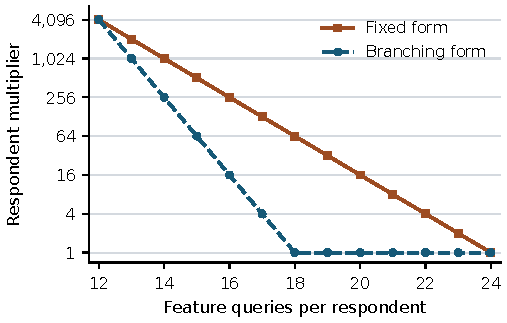
\includegraphics[width=.62\textwidth]{figures/query_cost.pdf}
\caption{Exact synthetic budget curve for the same update on 24 features ($k=6$). The fixed coefficient is 64 and the branching coefficient is one at 18 queries.}
\label{fig:cost}
\end{figure}


